\documentclass{article}
\usepackage[utf8]{inputenc}
\usepackage{amsmath, amssymb, amsfonts}
\usepackage{booktabs}
\usepackage{algorithm}
\usepackage{algpseudocode}
\usepackage{geometry}
\usepackage{hyperref}
\usepackage{graphicx}
\geometry{margin=1in}

\title{\textbf{Decompose, Analyze and Rethink:\\ Solving Intricate Problems with Human-like Reasoning Cycle}}

\author{
  \textbf{Shangzi Xue}$^1$, \textbf{Zhenya Huang}$^{1,2}$, \textbf{Jiayu Liu}$^1$, \textbf{Xin Lin}$^1$, \textbf{Yuting Ning}$^1$,\\
  \textbf{Binbin Jin}$^1$, \textbf{Xin Li}$^1$, \textbf{Qi Liu}$^{1,2,*}$ \\[2mm]
  \small $^1$State Key Laboratory of Cognitive Intelligence, University of Science and Technology of China \\
  \small $^2$Institute of Artificial Intelligence, Hefei Comprehensive National Science Center \\
  \small \texttt{\{xueshangzi, jy251198, linx, ningyt, bb0725\}@mail.ustc.edu.cn} \\
  \small \texttt{\{huangzhy, leexin, qiliuql\}@ustc.edu.cn}
}
\date{}

\begin{document}

\maketitle

\begin{abstract}
In this paper, we introduce DeAR (Decompose-Analyze-Rethink), a framework that iteratively builds a reasoning tree to tackle intricate problems within a single large language model (LLM). Unlike approaches that extend or search for rationales, DeAR is featured by 1) adopting a tree-based question decomposition manner to plan the organization of rationales, which mimics the logical planning inherent in human cognition; 2) globally updating the rationales at each reasoning step through natural language feedback. Specifically, the Decompose stage decomposes the question into simpler sub-questions, storing them as new nodes; the Analyze stage generates and self-checks rationales for sub-questions at each node level; and the Rethink stage updates parent-node rationales based on feedback from their child nodes. By generating and updating the reasoning process from a more global perspective, DeAR constructs more adaptive and accurate logical structures for complex problems, facilitating timely error correction compared to rationale-extension and search-based approaches such as Tree-of-Thoughts (ToT) and Graph-of-Thoughts (GoT). We conduct extensive experiments on three reasoning benchmarks, including ScienceQA, StrategyQA, and GSM8K, which cover a variety of reasoning tasks, demonstrating that our approach significantly reduces logical errors and enhances performance across various LLMs. Furthermore, we validate that DeAR is an efficient method that achieves a superior trade-off between accuracy and reasoning time compared to ToT and GoT.
\end{abstract}

\let\thefootnote\relax\footnote{$^*$Corresponding Author. 38th Conference on Neural Information Processing Systems (NeurIPS 2024).}

\section{Introduction}
Learning to perform intricate reasoning, including commonsense reasoning, knowledge reasoning, and mathematical reasoning, is a crucial step towards achieving general artificial intelligence. The tasks always present a significant challenge as they require many human-like intricate problem-solving abilities, such as abstract thinking and logical inference, which could consolidate many decision-making applications in real-world scenarios.

Recent advances have witnessed remarkable performances of scaled-up large language models (LLMs) in various reasoning tasks, including GPT, LLaMA, and ChatGLM. They could enable several state-of-the-art prompting approaches like Chain-of-Thought (CoT), Tree-of-Thoughts (ToT), Graph-of-Thoughts (GoT), etc., to enhancing reasoning capabilities. They not only improve problem-solving performance but also reveal their intrinsic reasoning steps (i.e., rationales) through linear, tree-based, or graph-based structures. For example, given a math problem, ToT maintains a tree of thoughts with intermediate nodes to generate the rationales step by step. Specifically, through several operations including exploration, termination, and traceback on the nodes, ToT ultimately identifies the complete reasoning path, leading to the answer.

However, although ToT and its variants perform the reasoning process explicitly, such a rationale-extension and search-based reasoning paradigm is still far from human-like intelligence and limits problem-solving abilities to some extent: On one hand, this tree-like structure is rigid and sometimes illogical. The ToT approaches often require setting a fixed number of thought branches each time it expands, which can result in either missing information or redundancy. Its reasoning process essentially extends previous rationales at each step, but falls short of the logical planning inherent in human thinking. On the other hand, ToT generates rationale paths sequentially, and errors along the path cannot be promptly corrected. This allows mistakes to propagate to subsequent steps, ultimately leading to an incorrect final outcome.

To address these challenges, we propose a novel reasoning paradigm \textbf{DeAR (Decompose-Analyze-Rethink)}, which enhances LLMs' capacity for complex problem-solving by emulating human reasoning. This approach is inspired by several theories in cognitive science. Specifically, reasoning simplification theory suggests that when confronted with an intricate question, humans tend to break it down into simpler ones, which help in organizing thoughts and solving problems more logically. By sequentially resolving these sub-questions and using their results as feedback to update answers for previously generated sub-questions, we ultimately arrive at the final answer.

To implement such a human-like problem-solving process, we introduce a \textbf{Decompose-Analyze-Rethink cycle}. This involves gradually constructing a reasoning tree guided by sub-questions, following a top-to-bottom reasoning process. The process begins with the \textbf{Decompose stage}, where a prompt-based method breaks down the question into simpler sub-questions at subsequent nodes. Then, the \textbf{Analyze stage} takes charge of problem-solving at the node level. The stage also introduces a self-check module to ensure the quality of the generated rationales, thus refines the reasoning process. Last, in the \textbf{Rethink stage}, the result at the current node is evaluated to determine if the reasoning in parent nodes requires further updates, providing a global perspective. After multiple cycles, the answer can be summarized from the root node.

\section{Related Work}
\subsection{Prompt-based Approaches in LLM Reasoning}
There has been a growing interest in LLM reasoning research, with various prompting schemes applied in areas such as commonsense, mathematical and knowledge reasoning, etc. Early methods appends examples on top of the input question (few-shot prompting or performs in-context learning (ICL)), or includes no examples at all (zero-shot prompting). Recent research has sought to enhance the capabilities of large language models (LLMs) by introducing intermediate reasoning steps into the prompting process, epitomized by methods such as the Chain-of-Thought (CoT). By prompting LLMs to solve problems step by step, the CoT method demonstrates outstanding performance in multi-step reasoning tasks. Self-consistency is a significant improvement upon CoT, where multiple CoT paths are initially generated, and the best one is selected as the final result. In parallel, other prompting methods design search-based schemes for LLMs, such as Tree-of-Thoughts (ToT) and Graph-of-Thoughts (GoT).

\subsection{Question Decomposition}
Question decomposition, which decomposes complex questions into multiple sub-ones, has been shown to largely improve models' reasoning ability. Early works decompose questions with hand-crafted rules and lexicon-syntactic features. These works heavily rely on human efforts, which are hard to extend to general domains and tasks. Recently, researchers utilize neural network models to decompose questions. More recently, in the era of LLMs, there are a lot of work exploring LLMs for question decomposition. These prompting-based question decomposition methods serve as an important step in reasoning and planning with LLMs.

\section{Problem Formulation and Preliminaries}
\subsection{Problem Definition}
In this paper, we focus on the intricate reasoning task. The input of the task is the question $Q$. The output is a rationale $R=(r_1, r_2, \dots, r_k)$ with $k$ word tokens, and the answer $A$ derived from $R$. Given the input question $Q$, we aim to design a reasoning framework with LLM backbone $p_\theta$ to generate the rationale $R$ and answer $A$ as outputs.

\begin{figure}[htbp]
    \centering
    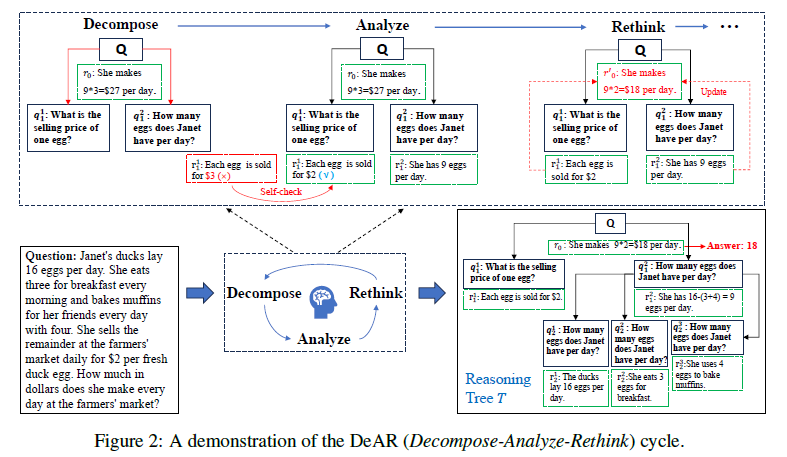
\includegraphics[width=0.8\textwidth]{figures/photo_1.png}
    \caption{Overview of the problem formulation and proposed reasoning process.}
    \label{fig:problem_overview}
\end{figure}

\subsection{Reasoning Tree}
Motivated by the reasoning simplification theory, we propose a novel reasoning structure for LLMs, named Reasoning Tree $T$. Overall, this Reasoning Tree decomposes and resolves sub-questions using a top-down approach, while concurrently updating existing solutions through a bottom-up process. Formally, the Reasoning Tree $T$ can be defined as $T=(N,E)$ where $N$ is the set of tree nodes and $E$ is the edge set. Each node $n=(q,r,s)\in N$ contains a question $q$ as a sub-question of the target $Q$, a rationale $r$ to $q$, and a score $s$ evaluating the logical coherence of $r$. Each directed edge $e=(n_p,n_c)\in E$ means that the upper-level sub-question $q_p$ in the parent node $n_p$ is decomposed into a lower-level one $q_c$ in the child node $n_c$.

\subsection{Framework Overview}
To construct the Reasoning Tree $T$, we propose a novel DeAR (Decompose-Analyze-Rethink) cycle as the core of our framework. The cycle is composed of three stages: Decompose, Analyze and Rethink. Specifically, in the Decompose stage, one upper-level question is decomposed into several lower-level ones. In the Analyze stage, the framework solves the newly generated sub-questions by generating and self-checking rationales. In the Rethink stage, the newly generated rationales are used to update existing ones in the parent nodes.

\section{DeAR (Decompose-Analyze-Rethink) Cycle}
Initially, the target question $Q$ is set as the question $q_0$ in the root node $n_0$. The framework selects an existing edge node $n_t=(q_t,r_t,s_t)$ (where $t$ is the level of the node) from $T$ to start the cycle. 

\subsection{Decompose Stage}
According to Analogical Reasoning theory, when humans conduct reasoning, they often analogize the logical processes of new questions to those of similar questions. Therefore, we select top-$K$ nearest neighbors from a human-annotated demonstration pool $P$ to form $K$ question-decomposition examples:
\begin{equation}
lh_Q = (Q_i^d, subqs^i) \quad (i=1,2,\dots,K)
\end{equation}
Given question $q_t$, if its coherence score $s_t$ is higher than a threshold $\epsilon_1$, we prompt the LLM to autonomously break it down into several sub-questions $\{q_{t+1}^j, j=1,\dots,J\}$:
\begin{equation}
\{q_{t+1}^j, j=1,\dots,J\} \leftarrow \text{Decompose}(p_\theta, h_1, lh_Q, q_t)
\end{equation}

\subsection{Analyze Stage}
In the Analyze stage, we reason the answers for all the sub-questions $\{q_{t+1}^j\}$ at level $t+1$:
\begin{equation}
r_{t+1}^j \leftarrow \text{Solve}(p_\theta, h_2, q_{t+1}^j)
\end{equation}
To address hallucination, we develop a self-check method that promptly identifies and corrects these errors:
\begin{equation}
\hat{r}_{t+1}^j \leftarrow \text{Self\_Check}(p_\theta, h_3, q_{t+1}^j, r_{t+1}^j)
\end{equation}
Then, we evaluate the logical coherence by generating a coherence score $s_{t+1}^j$:
\begin{equation}
s_{t+1}^j \leftarrow \text{Score}(p_\theta, h_4, q_{t+1}^j, \hat{r}_{t+1}^j)
\end{equation}

\subsection{Rethink Stage}
During the rethinking process, we use information from lower-level nodes to ``rethink'' higher-level nodes. If $s_{t+1}^j$ exceeds threshold $\epsilon_2$, we extract a subset of $k$ most related nodes $L_k$ from $L \triangleq \{n_l, l \le t\}$:
\begin{equation}
L_k \leftarrow \text{Extract}(p_\theta, h_5, L, q_{t+1}^j), \quad L_k \subseteq L
\end{equation}
Next, we use the rationale $\hat{r}_{t+1}^j$ to update the rationale $r$ of each extracted node $n_e$:
\begin{equation}
r' \leftarrow \text{Update}(p_\theta, h_6, n_e(q, r, s), \hat{r}_{t+1}^j)
\end{equation}
Finally, we replace $r$ with the updated rationale $r'$:
\begin{equation}
n_e(q, r', s) \leftarrow n_e(q, r, s)
\end{equation}

\begin{algorithm}[H]
\caption{Decompose-Analyze-Rethink}
\begin{algorithmic}[1]
\Input Question $Q$, Parameters $p_\theta$, Prompts $(h_1 \sim h_6)$, Thresholds $\epsilon_1, \epsilon_2$
\Output Rationale $R$, Answer $A$
\State Create an empty node queue $N$
\State Enqueue $n_0(q_0=Q, r_0=\text{None}, s_0=1)$ into $N$
\While{$N$ is not empty and current level $<$ max depth}
    \State Dequeue current node $n_t(q_t, r_t, s_t)$ from $N$
    \If{$n_t$ is an end node $n_{end}$}
        \State \textbf{continue}
    \ElseAction ~ \textbf{if} $s_t > \epsilon_1$ \textbf{then}
        \State // \textit{Stage 1: Decompose}
        \State $\{q_{t+1}^j\} \leftarrow \text{Decompose}(p_\theta, h_1, lh_Q, q_t)$
        \State // \textit{Stage 2: Analyze}
        \State $r_{t+1}^j \leftarrow \text{Solve}(p_\theta, h_2, q_{t+1}^j)$
        \State $\hat{r}_{t+1}^j \leftarrow \text{Self\_Check}(p_\theta, h_3, q_{t+1}^j, r_{t+1}^j)$
        \State $s_{t+1}^j \leftarrow \text{Score}(p_\theta, h_4, q_{t+1}^j, \hat{r}_{t+1}^j)$
        \State $n_{t+1}^j \leftarrow (q_{t+1}^j, \hat{r}_{t+1}^j, s_{t+1}^j)$
        \State Enqueue $n_{t+1}^j$ into $N$
        \State // \textit{Stage 3: Rethink}
        \If{$s_{t+1}^j > \epsilon_2$}
            \State $L_k \leftarrow \text{Extract}(p_\theta, h_5, L, q_{t+1}^j)$
            \State $r' \leftarrow \text{Update}(p_\theta, h_6, n_e(q,r,s), \hat{r}_{t+1}^j)$
            \State $n_e(q, r', s) \leftarrow n_e(q, r, s)$
        \Else
            \State Enqueue $n_{end}$ into $N$
        \EndIf
    \EndIf
\EndWhile
\State $R \leftarrow r_0$
\State Extract answer $A$ from $R$
\State \textbf{return} $R, A$
\end{algorithmic}
\end{algorithm}

\section{Experiments}
\subsection{Experimental Setup}
We employ ScienceQA, StrategyQA, and GSM8K datasets to evaluate knowledge, logical, and mathematical reasoning tasks respectively. Experiments are conducted using GPT-3.5, LLaMA2-7B, and ChatGLM3-6B backbones.

\subsection{Experimental Results}
\begin{table}[H]
\centering
\caption{Overall results of our DeAR Framework on three intricate reasoning datasets.}
\vspace{2mm}
\small
\begin{tabular}{lccccccccc}
\toprule
& \multicolumn{3}{c}{\textbf{ScienceQA}} & \multicolumn{3}{c}{\textbf{StrategyQA}} & \multicolumn{3}{c}{\textbf{GSM8K}} \\
\cmidrule(lr){2-4} \cmidrule(lr){5-7} \cmidrule(lr){8-10}
\textbf{Method} & \textbf{GPT-3.5} & \textbf{LLaMA2} & \textbf{ChatGLM3} & \textbf{GPT-3.5} & \textbf{LLaMA2} & \textbf{ChatGLM3} & \textbf{GPT-3.5} & \textbf{LLaMA2} & \textbf{ChatGLM3} \\
\midrule
Few-shot & 73.97 & 66.35 & 42.46 & 67.71 & 61.21 & 54.41 & 74.26 & 72.25 & 51.02 \\
CoT & 75.17 & 67.58 & 46.35 & 69.26 & 63.86 & 57.18 & 79.55 & 74.04 & 53.85 \\
ToT & 82.52 & 69.01 & 49.58 & 71.89 & 66.52 & 59.21 & 83.42 & 75.22 & 55.88 \\
GoT & 82.34 & 68.86 & 49.26 & 72.02 & 66.61 & 59.88 & 84.77 & 75.95 & 56.01 \\
\textbf{DeAR} & \textbf{83.68} & \textbf{70.57}$^*$ & \textbf{51.08}$^*$ & \textbf{73.36} & \textbf{68.33} & \textbf{61.02} & \textbf{86.82} & \textbf{78.01}$^*$ & \textbf{58.54} \\
\midrule
Least-to-most & 76.61 & 68.02 & 47.45 & 70.55 & 64.43 & 58.36 & 81.25 & 74.67 & 54.21 \\
SelfCheck & 75.81 & 69.33 & 49.23 & 68.87 & 66.35 & 61.22 & 79.88 & 75.28 & 56.72 \\
\bottomrule
\end{tabular}
\end{table}

\begin{table}[H]
\centering
\caption{Characteristics of $T$ in different datasets.}
\vspace{2mm}
\begin{tabular}{lccc}
\toprule
\textbf{Metric} & \textbf{ScienceQA} & \textbf{StrategyQA} & \textbf{GSM8K} \\
\midrule
Avg Branch & 1.58 & 2.43 & 2.06 \\
Avg Depth & 3.62 & 1.96 & 2.55 \\
Avg Length of R & 66.34 & 61.55 & 85.27 \\
\bottomrule
\end{tabular}
\end{table}

\section{Conclusion}
In this paper, we introduced DeAR (Decompose-Analyze-Rethink), a framework designed to mimic human reasoning patterns in tackling intricate problems by constructing a reasoning tree in a top-down, iterative manner. Extensive experiments demonstrate that DeAR improves reasoning performance across different LLMs and surpasses state-of-the-art methods like ToT and GoT in logical coherence and accuracy.

\end{document}